% =============================================================================
%  동적 프로그래밍 — 『밑바닥부터 시작하는 딥러닝 4』 4장 정리
%
%  컴파일:  tectonic -X compile ch04_dp.tex
%  (XeLaTeX 계열 엔진 + kotex + NanumGothic 필요)
%  그림:    python ch04/paper/fig_convergence.py  로 fig_convergence.png 생성
% =============================================================================
\documentclass[11pt,a4paper]{article}

\usepackage{kotex}
\usepackage{amsmath,amssymb}
\usepackage{amsthm}
\usepackage{graphicx}
\usepackage{booktabs}
\usepackage{multirow}
\usepackage{listings}
\usepackage{xcolor}
\usepackage{algorithm}
\usepackage{algpseudocode}
\usepackage[margin=27mm,top=28mm,bottom=28mm]{geometry}
\usepackage[labelsep=period,font=small,labelfont=bf]{caption}
\usepackage{enumitem}
\usepackage[hidelinks]{hyperref}

% ---- 한글 글꼴 -------------------------------------------------------------
\setmainhangulfont{NanumGothic}
\setsanshangulfont{NanumGothic}
\setmonohangulfont[Scale=MatchLowercase]{NanumGothic}

% ---- 한글 캡션 이름 ---------------------------------------------------------
\renewcommand{\figurename}{그림}
\renewcommand{\tablename}{표}
\renewcommand{\refname}{참고문헌}
\renewcommand{\abstractname}{초록}
\renewcommand{\contentsname}{차례}
\floatname{algorithm}{알고리즘}
\renewcommand{\algorithmicrequire}{\textbf{입력:}}
\renewcommand{\algorithmicensure}{\textbf{출력:}}

% ---- 정리 환경 -------------------------------------------------------------
\newtheorem{proposition}{명제}
\newtheorem{corollary}[proposition]{따름정리}
\renewcommand{\proofname}{증명}

% ---- 코드 리스팅 -----------------------------------------------------------
\definecolor{codekw}{RGB}{0,86,153}
\definecolor{codecm}{RGB}{112,128,144}
\definecolor{codestr}{RGB}{163,21,21}
\definecolor{codebg}{RGB}{249,249,250}
% 주의: listings는 라틴 문자를 단어 단위로 버퍼링했다가 출력하는데, kotex 환경에서
% 한글이 섞이면 버퍼가 한글 뒤에 flush되어 글자 순서가 뒤바뀐다("q에" -> "에q").
% 그래서 한글 주석은 escapeinside 구간에서 일반 조판 모드로 넘겨 처리한다.
\lstdefinestyle{py}{
  language=Python,
  escapeinside={<@}{@>},
  basicstyle=\ttfamily\small,
  keywordstyle=\color{codekw}\bfseries,
  commentstyle=\color{codecm}\itshape,
  stringstyle=\color{codestr},
  backgroundcolor=\color{codebg},
  frame=single,
  rulecolor=\color{black!25},
  framesep=5pt,
  columns=fullflexible,
  keepspaces=true,
  showstringspaces=false,
  breaklines=true,
  captionpos=b,
  numbers=none,
  aboveskip=1.1em,
  belowskip=0.6em,
}
\lstset{style=py}
\renewcommand{\lstlistingname}{코드}

% ---- 그림 경로 -------------------------------------------------------------
\graphicspath{{../../images/figures/}{../../images/equations/}{./}}

% ---- 편의 매크로 -----------------------------------------------------------
\newcommand{\E}{\mathbb{E}}
\newcommand{\Sset}{\mathcal{S}}
\newcommand{\Aset}{\mathcal{A}}
\newcommand{\Lone}{\texttt{L1}}
\newcommand{\Ltwo}{\texttt{L2}}
\newcommand{\Tpi}{\mathcal{T}_\pi}
\newcommand{\Tstar}{\mathcal{T}_*}
\newcommand{\bookfig}[1]{\textit{출처: 원서 그림 #1.}}
\newcommand{\cmt}[1]{\textcolor{codecm}{#1}}   % 리스팅 안의 한글 주석

\title{\bfseries 동적 프로그래밍\\[2mm]
\large 벨만 방정식의 등호를 갱신식으로 바꾸기: 정책 반복법과 가치 반복법,
그리고 ``평가를 얼마나 끝까지 돌리는가''라는 하나의 축}
\author{sajacaros\\\small \texttt{sajacall82@naver.com}}
\date{2026년 8월 23일}

\begin{document}
\maketitle

\begin{abstract}
\noindent
앞 장에서 벨만 방정식을 얻었지만 그것을 실제로 푸는 방법은 두 칸짜리 예제에서 손으로 연립방정식을
세우는 것뿐이었고, 직접 해법은 $O(|\Sset|^3)$의 벽에 부딪힌다. \emph{동적 프로그래밍}(DP)은 이 방정식의
등호를 대입으로 바꿔 읽는다. 우변에 현재 추정치 $V_k$를 넣어 좌변 $V_{k+1}$을 얻기를 반복하면, 축소
사상의 성질에 의해 참값으로 수렴한다.
본고는 이 착상에서 출발하여 \emph{반복적 정책 평가}, \emph{정책 반복법}, \emph{가치 반복법}의 세
알고리즘을 정리하고, 세 알고리즘이 ``평가를 얼마나 끝까지 돌리는가''라는 하나의 축 위의 서로 다른
지점임을 보인다.
원서\cite{dlfs4} 4장의 예제 여섯 편을 소재로 삼되 여기에 네 가지 정량 분석을 더하였다.
첫째, 배열 하나로 제자리 갱신하는 구현이 배열 둘을 쓰는 구현보다 빠른(76회 대 60회) 이유가
\emph{야코비 반복과 가우스-자이델 반복}의 차이임을 밝히고, 두 반복 행렬의 스펙트럼 반지름을
$0.9000$과 $0.8696$으로 계산하여 반복 횟수의 비 $0.754$를 예측하고 실측이 문턱을 낮출수록
이 값에 접근함을 확인한다.
둘째, 정지 문턱 $\varepsilon$이 남기는 오차의 상한이 $\gamma\varepsilon/(1-\gamma)$이며, 두 칸 세계의
야코비 갱신에서는 이 상한이 \emph{등호로 달성}됨을 증명하고 실측($8.325\times10^{-4}$)으로 확인한다.
나아가 앞 장의 표(정확해)와 이 장의 표(문턱 $10^{-3}$)가 세 칸에서 소수 둘째 자리까지 다른 것이 바로
이 오차임을 보인다.
셋째, 정책 반복법과 가치 반복법의 비용을 스윕 수로 환산하여 32회 대 4회, 백업 횟수로 1776회 대
240회임을 제시한다.
넷째, 이 환경의 최적 가치가 $v_*(s)=\gamma^{d(s)-1}$이라는 닫힌 형태를 가짐을 증명하고, 그로부터
가치 반복법이 유한 스윕 안에 \emph{정확히} 끝남을 보인다.

\vspace{2mm}
\noindent\textbf{주제어:} 강화 학습, 동적 프로그래밍, 반복적 정책 평가, 정책 반복법, 가치 반복법,
가우스-자이델 반복, 일반화된 정책 반복
\end{abstract}

\tableofcontents
\vspace{4mm}

% =============================================================================
\section{서론}
% =============================================================================

\subsection{연립방정식에서 반복 계산으로}

앞 장\cite{ch03}에서 벨만 방정식
\begin{equation}
  v_\pi(s) = \sum_{a} \pi(a\mid s) \sum_{s'} p(s'\mid s,a)
             \bigl\{\, r(s,a,s') + \gamma\, v_\pi(s') \,\bigr\}
  \label{eq:bellman}
\end{equation}
을 얻었고, 이것이 $v_\pi$에 대한 연립일차방정식이므로 $(I-\gamma P_\pi)v = r_\pi$를 풀면 정확해가
나온다는 것도 확인하였다. 그러나 그 방법은 $|\Sset|\times|\Sset|$ 행렬을 실체화해야 하므로 연산량이
$O(|\Sset|^3)$, 기억 용량이 $O(|\Sset|^2)$로 늘어난다. 앞 장에서 계산한 손익분기는 $\gamma=0.9$,
$\varepsilon=10^{-10}$에서 약 51개 상태였다.

\begin{figure}[htbp]
\centering
\includegraphics[width=0.72\linewidth]{{fig 4-1}.png}
\caption{앞 장에서 한 일. 환경 모델 $(p,r)$과 정책 $\pi$를 벨만 방정식에 넣고 가운데 주황 상자
``연립방정식 계산기''로 가치 함수를 얻었다. 이 장에서는 그 상자를 \emph{반복 계산}으로 바꾼다.
\bookfig{4-1}}
\label{fig:solver}
\end{figure}

이 장이 바꾸는 것은 그림~\ref{fig:solver}의 가운데 상자 하나다. 착상은 한 줄로 요약된다.
\emph{식~\eqref{eq:bellman}의 등호를 대입으로 바꿔 읽는다.} 우변에 현재의 추정치 $V_k$를 넣고 좌변을
새 추정치 $V_{k+1}$로 삼는 것이다.
\begin{equation}
  V_{k+1}(s) = \sum_{a} \pi(a\mid s) \sum_{s'} p(s'\mid s,a)
               \bigl\{\, r(s,a,s') + \gamma\, V_k(s') \,\bigr\}.
  \label{eq:update}
\end{equation}
참값 $v_\pi$가 아니라 추정치임을 나타내기 위해 대문자 $V$를 쓴다. 앞 장에서 증명했듯 이 갱신을 정의하는
벨만 연산자는 $\gamma$-축소 사상이므로, 아무 값에서 출발해도 유일한 고정점 $v_\pi$로 수렴한다.

이 장의 목표는 이 갱신을 뼈대로 삼아 두 알고리즘을 세우는 것이다. \emph{정책 반복법}은 평가와 개선을
번갈아 반복하고, \emph{가치 반복법}은 둘을 하나로 합쳐 최적 가치를 직접 구한다. 두 알고리즘 모두
환경 모델 $p$와 $r$를 완전히 알고 있다고 전제하며, 이 전제가 깨지는 것이 다음 장부터다.

\subsection{본고의 구성과 기여}

2절에서 반복적 정책 평가를 두 칸짜리 그리드 월드에 적용하며 두 가지 구현을 비교한다. 3절에서
$3\times4$ 그리드 월드로 옮겨 가고, 4절과 5절에서 각각 정책 반복법과 가치 반복법을 다룬다.

원서 4장은 예제 코드를 제공하므로 본고는 그것을 그대로 쓰되, 다음 네 가지 분석을 더하였다.

\begin{enumerate}[leftmargin=*,itemsep=2pt]
  \item \textbf{제자리 갱신이 빠른 이유}(\S\ref{sec:gs}). 원서는 배열 하나를 쓰는 구현이 $76$회에서
        $60$회로 줄어든다는 사실을 관찰로 제시한다. 본고는 이것이 수치해석의 \emph{야코비 반복}과
        \emph{가우스-자이델 반복}의 차이임을 밝히고, 두 반복 행렬의 스펙트럼 반지름
        $0.9000$과 $0.8696$에서 반복 횟수의 비 $0.754$를 예측한 뒤 실측이 문턱을 낮출수록 그 값에
        접근함을 보인다.
  \item \textbf{정지 문턱이 남기는 오차}(\S\ref{sec:threshold}). 상한
        $\gamma\varepsilon/(1-\gamma)$를 증명하고, 두 칸 세계의 야코비 갱신에서는 이 상한이 등호로
        달성됨을 보인다. 나아가 앞 장의 표(정확해)와 이 장의 표(문턱 $10^{-3}$)가 세 칸에서 소수
        둘째 자리까지 다른 것이 바로 이 오차임을 확인한다.
  \item \textbf{두 알고리즘의 실제 비용}(\S\ref{sec:cost}). 원서의 비교표는 정책 반복법을
        ``사이클 5회'', 가치 반복법을 ``스윕 4회''로 적는데, 단위가 달라 그대로 견줄 수 없다. 같은
        단위로 환산하면 32 스윕 대 4 스윕, 백업 횟수로는 1776회 대 240회다.
  \item \textbf{최적 가치의 닫힌 형태와 유한 수렴}(\S\ref{sec:closed}).
        $v_*(s)=\gamma^{d(s)-1}$($d$는 폭탄 칸을 지나지 않는 최단 걸음 수)임을 증명하고, 그로부터
        가치 반복법이 문턱과 무관하게 유한 스윕 안에 정확히 끝남을 보인다. 제자리 갱신은 3스윕,
        동기 갱신은 5스윕이 걸린다.
\end{enumerate}

% =============================================================================
\section{반복적 정책 평가}
% =============================================================================

\subsection{등호를 갱신식으로}

소재는 앞 장에서 쓴 두 칸짜리 그리드 월드다. 정책은 $\Lone$과 $\Ltwo$ 어디에서나 \texttt{Left}와
\texttt{Right}를 $0.5$씩 고르는 무작위 정책이고 $\gamma=0.9$다. 상태 전이가 결정적이므로
식~\eqref{eq:update}에서 안쪽 합이 사라진다.
\begin{equation}
  V_{k+1}(s) = \sum_{a} \pi(a\mid s)
               \bigl\{\, r\bigl(s,a,f(s,a)\bigr) + \gamma\, V_k\bigl(f(s,a)\bigr) \,\bigr\}.
  \label{eq:update-det}
\end{equation}
이 갱신을 반복하는 것을 \emph{반복적 정책 평가}(iterative policy evaluation)라 한다.

\begin{figure}[htbp]
\centering
\begin{minipage}[t]{0.50\linewidth}\centering
  \includegraphics[width=\linewidth]{{fig 4-4}.png}
\end{minipage}\hfill
\begin{minipage}[t]{0.46\linewidth}\centering
  \includegraphics[width=\linewidth]{{fig 4-5}.png}
\end{minipage}
\caption{$\Lone$의 갱신을 그린 백업 다이어그램(왼쪽)과 $V_0=(0,0)$에서 한 번 갱신한 결과(오른쪽).
$V_1(\Lone)$이 여전히 $0$인 것은 $-1$과 $+1$이 반반이라 상쇄되기 때문이고,
$V_1(\Ltwo)=0.5\times0+0.5\times(-1)=-0.5$다. 참값 $(-2.25,-2.75)$와는 아직 멀다. \bookfig{4-4, 4-5}}
\label{fig:first-update}
\end{figure}

그림~\ref{fig:first-update}의 갱신을 식으로 쓰면 다음과 같다.
\begin{align}
  V_{k+1}(\Lone) &= 0.5\bigl\{-1 + 0.9\,V_k(\Lone)\bigr\} + 0.5\bigl\{\,1 + 0.9\,V_k(\Ltwo)\bigr\},
  \label{eq:l1-update}\\
  V_{k+1}(\Ltwo) &= 0.5\bigl\{\;\;0 + 0.9\,V_k(\Lone)\bigr\} + 0.5\bigl\{-1 + 0.9\,V_k(\Ltwo)\bigr\}.
  \label{eq:l2-update}
\end{align}

\paragraph{언제 멈추는가.}
참값을 모르므로 ``더 이상 거의 변하지 않는다''를 수렴의 신호로 삼는다. 한 번의 갱신에서 가장 크게 변한
양을
\begin{equation}
  \delta_k = \bigl\|V_k - V_{k-1}\bigr\|_\infty = \max_{s}\,\bigl|V_k(s)-V_{k-1}(s)\bigr|
  \label{eq:delta}
\end{equation}
로 두고 $\delta_k<\varepsilon$이면 종료한다. 이 규칙이 실제로 얼마의 오차를 남기는지는
\S\ref{sec:threshold}에서 따로 따진다.

\subsection{두 가지 구현: 배열 둘과 제자리}

식~\eqref{eq:l1-update}, \eqref{eq:l2-update}을 코드로 옮기는 방법은 두 가지다. 하나는 식을 글자
그대로 옮겨 옛 배열 $V$를 읽고 새 배열 \texttt{new\_V}에 쓰는 것이다.

\begin{lstlisting}[caption={배열 두 개를 쓰는 구현 (\texttt{s01\_dp.py})},label={lst:two-array}]
V = {'L1': 0.0, 'L2': 0.0}
new_V = V.copy()
while True:
    new_V['L1'] = 0.5 * (-1 + 0.9 * V['L1']) + 0.5 * (1 + 0.9 * V['L2'])
    new_V['L2'] = 0.5 * ( 0 + 0.9 * V['L1']) + 0.5 * (-1 + 0.9 * V['L2'])
    delta = max(abs(new_V['L1'] - V['L1']), abs(new_V['L2'] - V['L2']))
    V = new_V.copy()               <@\cmt{\# 한 스윕이 끝난 뒤에 통째로 교체}@>
    if delta < 0.0001:
        break
\end{lstlisting}

다른 하나는 배열 하나만 두고 계산하는 즉시 덮어쓰는 것이다.

\begin{lstlisting}[caption={제자리 갱신 구현 (\texttt{s02\_dp\_inplace.py})},label={lst:in-place}]
V = {'L1': 0.0, 'L2': 0.0}
while True:
    t = 0.5 * (-1 + 0.9 * V['L1']) + 0.5 * (1 + 0.9 * V['L2'])
    delta = abs(t - V['L1']); V['L1'] = t          <@\cmt{\# 여기서 곧바로 덮어씀}@>
    t = 0.5 * ( 0 + 0.9 * V['L1']) + 0.5 * (-1 + 0.9 * V['L2'])   <@\cmt{\# 방금 바뀐 값을 씀}@>
    delta = max(delta, abs(t - V['L2'])); V['L2'] = t
    if delta < 0.0001:
        break
\end{lstlisting}

\begin{figure}[htbp]
\centering
\begin{minipage}[t]{0.48\linewidth}\centering
  \includegraphics[width=\linewidth]{{fig 4-6}.png}
\end{minipage}\hfill
\begin{minipage}[t]{0.48\linewidth}\centering
  \includegraphics[width=\linewidth]{{fig 4-7}.png}
\end{minipage}
\caption{두 구현의 갱신 방식. 왼쪽은 화살표의 출발점이 항상 위쪽 $V$ 배열이므로 한 스윕 동안 $V$가
고정된다. 오른쪽은 화살표가 같은 배열 안에서 돌아오므로 방금 갱신된 값이 같은 스윕 안에서 다음 계산에
쓰인다. \bookfig{4-6, 4-7}}
\label{fig:two-impl}
\end{figure}

두 구현은 같은 답에 이르지만 걸리는 스윕 수가 다르다. 표~\ref{tab:two-impl}이 실행 결과다.

\begin{table}[htbp]
\centering
\caption{두 구현의 실행 결과($\varepsilon=10^{-4}$, $\gamma=0.9$). 참값은 $(-2.25,-2.75)$다.
마지막 열의 뜻은 \S\ref{sec:threshold}에서 다룬다.}
\label{tab:two-impl}
\small
\begin{tabular}{@{}llrrll@{}}
\toprule
구현 & 결과 $(\Lone,\Ltwo)$ & 스윕 & 최종 $\delta$ & 실제 오차 & 상한 $\gamma\delta/(1-\gamma)$ \\
\midrule
배열 둘 (\texttt{s01})   & $(-2.249168,\,-2.749168)$ & $76$ & $9.250\times10^{-5}$ & $8.325\times10^{-4}$ & $8.325\times10^{-4}$ \\
제자리 (\texttt{s02})    & $(-2.249378,\,-2.749420)$ & $60$ & $9.320\times10^{-5}$ & $6.218\times10^{-4}$ & $8.388\times10^{-4}$ \\
\bottomrule
\end{tabular}
\end{table}

제자리 갱신이 $76$회에서 $60$회로 줄었고 배열도 하나만 쓴다. 원서는 ``새 값이 곧바로 다음 계산에
반영되기 때문''이라는 설명에서 멈추는데, 다음 절에서 이 현상에 이름과 숫자를 붙인다.

\subsection{[보충] 제자리 갱신이 빠른 이유: 야코비와 가우스-자이델}
\label{sec:gs}

두 구현의 차이는 강화 학습에 고유한 것이 아니라 선형 방정식을 반복법으로 푸는 고전적인 두 방식의
차이다. 벨만 방정식을 행렬로 쓰면 $v = r_\pi + \gamma P_\pi v$이고, 상태를 스윕 순서대로 번호 매겨
$P_\pi = L + D + U$($L$은 대각선 아래, $D$는 대각선, $U$는 대각선 위)로 분해하면 두 구현은 각각
다음 갱신에 대응한다.
\begin{align}
  \text{배열 둘:}\quad & V_{k+1} = r_\pi + \gamma P_\pi V_k,
  &&M_{\mathrm{J}} = \gamma P_\pi, \label{eq:jacobi}\\
  \text{제자리:}\quad & V_{k+1} = r_\pi + \gamma\bigl(L\,V_{k+1} + (D+U)\,V_k\bigr),
  &&M_{\mathrm{GS}} = (I-\gamma L)^{-1}\gamma(D+U). \label{eq:gs}
\end{align}
앞의 것이 \emph{야코비 반복}, 뒤의 것이 \emph{가우스-자이델 반복}이다. 식~\eqref{eq:gs}에서
$V_{k+1}$이 우변에도 나타나는 것은 순환 참조가 아니라, $L$이 대각선 아래만 채우므로 $s$번째 성분을
계산할 때 이미 갱신이 끝난 $1,\dots,s-1$번째 성분만 쓴다는 뜻이다. 이것이 코드에서
\lstinline|V['L1']|을 덮어쓴 뒤 그 값을 \lstinline|V['L2']| 계산에 쓰는 두 줄에 대응한다.

두 방식의 수렴 속도는 각 반복 행렬의 스펙트럼 반지름이 결정한다. 두 칸 세계의
$P_\pi=\bigl(\begin{smallmatrix}0.5&0.5\\0.5&0.5\end{smallmatrix}\bigr)$에 대해
\begin{equation}
  M_{\mathrm{GS}} = \begin{pmatrix}1&0\\0.45&1\end{pmatrix}
                    \begin{pmatrix}0.45&0.45\\0&0.45\end{pmatrix}
                  = \begin{pmatrix}0.4500&0.4500\\0.2025&0.6525\end{pmatrix}
\end{equation}
이고, 두 스펙트럼 반지름은
\begin{equation}
  \rho(M_{\mathrm{J}}) = \gamma\,\rho(P_\pi) = 0.900000,
  \qquad
  \rho(M_{\mathrm{GS}}) = 0.869647
\end{equation}
이다. 앞의 값이 정확히 $\gamma$인 것은 $P_\pi$가 행 확률 행렬이라 $\rho(P_\pi)=1$이기 때문이며, 이는
앞 장에서 확인한 사실이다. 오차가 $k$스윕 뒤 $\rho^k$로 줄어드므로 같은 정확도에 이르는 데 필요한
스윕 수의 비는
\begin{equation}
  \frac{K_{\mathrm{GS}}}{K_{\mathrm{J}}}
  \;\longrightarrow\;
  \frac{\ln \rho(M_{\mathrm{J}})}{\ln \rho(M_{\mathrm{GS}})}
  = \frac{\ln 0.900000}{\ln 0.869647} = 0.7544
  \label{eq:ratio}
\end{equation}
로 점근한다. 표~\ref{tab:gs}가 실측이다.

\begin{table}[htbp]
\centering
\caption{정지 문턱에 따른 두 구현의 스윕 수. 문턱을 낮출수록 실측 비가
식~\eqref{eq:ratio}의 점근값 $0.7544$에 접근한다. $\varepsilon=10^{-4}$ 행이 표~\ref{tab:two-impl}의
$76$과 $60$이다.}
\label{tab:gs}
\small
\begin{tabular}{@{}lrrr@{}}
\toprule
$\varepsilon$ & 배열 둘(야코비) & 제자리(가우스-자이델) & 실측 비 \\
\midrule
$10^{-2}$ & $32$  & $27$  & $0.8438$ \\
$10^{-3}$ & $54$  & $44$  & $0.8148$ \\
$10^{-4}$ & $76$  & $60$  & $0.7895$ \\
$10^{-6}$ & $119$ & $93$  & $0.7815$ \\
$10^{-8}$ & $163$ & $126$ & $0.7730$ \\
\midrule
\multicolumn{3}{@{}l}{점근값 $\ln\rho(M_{\mathrm{J}})/\ln\rho(M_{\mathrm{GS}})$} & $0.7544$ \\
\bottomrule
\end{tabular}
\end{table}

문턱이 클 때 실측 비가 점근값보다 큰 것은 초기 몇 스윕의 과도 구간이 전체에서 차지하는 비중이 크기
때문이다. 문턱을 낮출수록 점근 영역이 길어져 비가 식~\eqref{eq:ratio}로 수렴한다.
그림~\ref{fig:convergence} 왼쪽이 이 관계를 로그 눈금에서 직접 보여준다. 두 곡선 모두 직선이고 그
기울기가 각각 $\ln\rho(M_{\mathrm{J}})$와 $\ln\rho(M_{\mathrm{GS}})$이며, 점선으로 겹쳐 그린 예측이
곡선과 구별되지 않는다.

\begin{figure}[htbp]
\centering
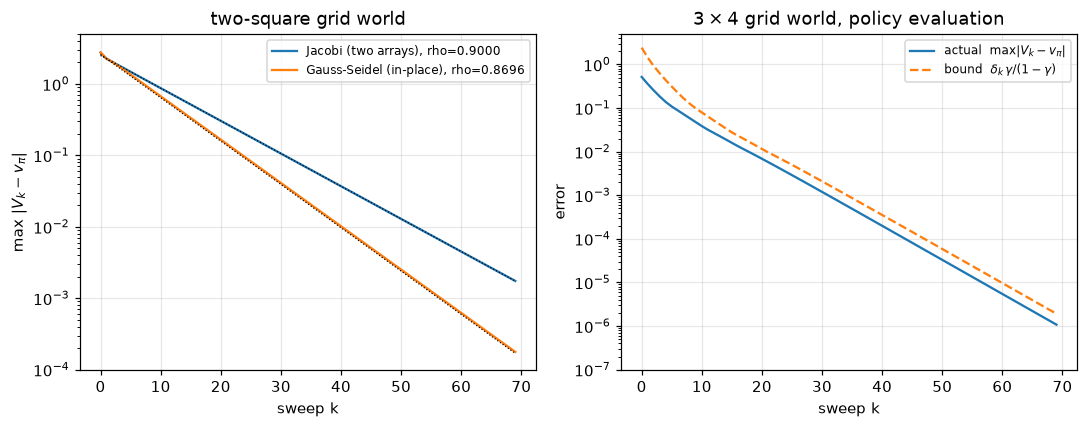
\includegraphics[width=\linewidth]{fig_convergence.png}
\caption{왼쪽: 두 칸 세계에서 야코비와 가우스-자이델 갱신의 오차(로그 눈금). 점선은 각 반복 행렬의
스펙트럼 반지름이 예측하는 직선으로, 곡선과 겹쳐 구별되지 않는다. 오른쪽: $3\times4$ 그리드의 반복적
정책 평가에서 실제 오차와 명제~\ref{prop:bound}의 상한. 상한이 언제나 위에 있고 두 선이 나란하다.
\texttt{ch04/paper/fig\_convergence.py}에서 생성.}
\label{fig:convergence}
\end{figure}

가우스-자이델의 이점이 공짜는 아니라는 점도 적어 둘 만하다. 식~\eqref{eq:gs}는 상태의 번호 매김,
즉 스윕 순서에 의존하므로 순서를 바꾸면 $\rho(M_{\mathrm{GS}})$도 바뀐다. 또 $V_{k+1}$이 자기 자신을
참조하므로 상태들을 병렬로 갱신할 수 없다. 야코비 갱신은 순서에 무관하고 완전히 병렬화되지만 배열이
둘 필요하다. 이 절의 결론은 ``제자리가 항상 낫다''가 아니라 ``이 예제에서 $76\to60$은 우연이 아니라
$\rho$의 차이로 설명된다''는 것이다.

\subsection{[보충] 정지 문턱이 남기는 오차}
\label{sec:threshold}

$\delta_k<\varepsilon$에서 멈추면 참값과 얼마나 떨어져 있는가. $\delta_k$는 참값과의 거리가 아니라
\emph{직전 추정치와의} 거리이므로 이 물음은 자명하지 않다. 답은 다음과 같다.

\begin{proposition}[정지 규칙의 오차 상한]
\label{prop:bound}
$\Tpi$가 $\gamma$-축소 사상이고 $V_k = \Tpi V_{k-1}$이면
\begin{equation}
  \bigl\|V_k - v_\pi\bigr\|_\infty
  \;\le\; \frac{\gamma}{1-\gamma}\,\bigl\|V_k - V_{k-1}\bigr\|_\infty
  = \frac{\gamma}{1-\gamma}\,\delta_k .
  \label{eq:stop-bound}
\end{equation}
\end{proposition}
\begin{proof}
$v_\pi$가 $\Tpi$의 고정점이므로
$\|V_k - v_\pi\| = \|\Tpi V_{k-1} - \Tpi v_\pi\| \le \gamma\|V_{k-1}-v_\pi\|$이고,
삼각부등식으로 $\|V_{k-1}-v_\pi\| \le \|V_{k-1}-V_k\| + \|V_k - v_\pi\|$이다. 두 식을 합치면
$(1-\gamma)\|V_k-v_\pi\| \le \gamma\|V_k-V_{k-1}\|$이 된다.
\end{proof}

$\gamma=0.9$이면 계수가 $\gamma/(1-\gamma)=9$이므로, 문턱이 $10^{-4}$라도 오차는 그 아홉 배까지
허용된다. 표~\ref{tab:two-impl}의 배열 둘 구현이 정확히 그 경계에 있다. 실제 오차
$8.325\times10^{-4}$가 상한 $9\times9.250\times10^{-5}=8.325\times10^{-4}$과 유효숫자 네 자리까지
같다. 우연이 아니다.

\begin{proposition}[두 칸 세계의 야코비 갱신에서는 상한이 등호로 달성된다]
\label{prop:tight}
$V_0=0$에서 출발한 식~\eqref{eq:jacobi}의 갱신에 대해, 두 칸 세계에서는 모든 $k\ge2$에 대해
식~\eqref{eq:stop-bound}이 등호로 성립한다.
\end{proposition}
\begin{proof}
앞 장에서 보았듯 오차는 $e_k = (\gamma P_\pi)^k e_0 = \gamma^k P_\pi^k e_0$이고, 이 환경의 $P_\pi$는
$P_\pi^2=P_\pi$인 사영 행렬이며 $e_0=-v_\pi$의 $\mathbf{1}$ 방향 성분이 $c=2.5$다. 따라서 $k\ge1$에서
$e_k = \gamma^k c\,\mathbf{1}$이므로 $\|e_k\|_\infty = \gamma^k c$이고
\begin{equation*}
  \delta_k = \|V_k - V_{k-1}\|_\infty = \|e_k - e_{k-1}\|_\infty
           = c\,\gamma^{k-1}(1-\gamma).
\end{equation*}
두 값의 비가 $\gamma^k c \big/ \bigl(c\gamma^{k-1}(1-\gamma)\bigr) = \gamma/(1-\gamma)$이다.
\end{proof}

명제~\ref{prop:tight}은 원서 4.1.2절이 ``오차 $\approx$ $\delta\times9$''라고 적은 것이 이 환경에서는
근사가 아니라 등식임을 말한다. 반면 제자리 갱신의 오차 $6.218\times10^{-4}$는 상한
$8.388\times10^{-4}$보다 작다. 가우스-자이델의 오차는 $\mathbf{1}$ 방향으로 정렬되지 않으므로 등호
조건을 만족하지 않기 때문이다.

\paragraph{앞 장의 표와 이 장의 표는 왜 다른가.}
이 상한은 두 장을 잇는 곳에서 눈에 보이는 차이를 만든다. 앞 장은 $3\times4$ 그리드의 무작위 정책
가치를 연립방정식으로 정확히 풀었고, 이 장은 같은 값을 문턱 $10^{-3}$의 반복 계산으로 구한다. 두
결과를 소수 둘째 자리로 반올림하면 세 칸에서 값이 다르다.

\begin{table}[htbp]
\centering
\caption{같은 문제, 다른 표. 앞 장의 정확해와 이 장의 반복 계산($\varepsilon=10^{-3}$, 23스윕)이
세 칸에서 소수 둘째 자리까지 갈린다. 차이는 모두 실제 오차 $4.877\times10^{-3}$ 안에 있다.}
\label{tab:mismatch}
\small
\begin{tabular}{@{}lrrr@{}}
\toprule
상태 & 앞 장(정확해) & 이 장(문턱 $10^{-3}$) & 차이 \\
\midrule
$(0,1)$ & $0.09$  & $0.10$  & $+0.0032$ \\
$(2,2)$ & $-0.44$ & $-0.43$ & $+0.0025$ \\
$(2,3)$ & $-0.79$ & $-0.78$ & $+0.0019$ \\
\bottomrule
\end{tabular}
\end{table}

표~\ref{tab:mismatch}의 차이는 모두 양수다. $V_0=0$에서 출발했고 이 문제의 참값이 대부분 음수이므로
추정치가 위에서 아래로 내려오는 중이기 때문이다. 표~\ref{tab:threshold}가 문턱을 낮출 때 이 오차가
어떻게 줄어드는지 보여준다.

\begin{table}[htbp]
\centering
\caption{$3\times4$ 그리드의 반복적 정책 평가에서 문턱, 스윕 수, 오차의 관계($\gamma=0.9$).
실제 오차가 모든 행에서 명제~\ref{prop:bound}의 상한 아래에 있고 대략 그 $0.6$배다.}
\label{tab:threshold}
\small
\begin{tabular}{@{}lrlll@{}}
\toprule
$\varepsilon$ & 스윕 & 최종 $\delta$ & 실제 오차 & 상한 $\gamma\delta/(1-\gamma)$ \\
\midrule
$10^{-2}$  & $11$  & $8.818\times10^{-3}$  & $3.858\times10^{-2}$  & $7.936\times10^{-2}$ \\
$10^{-3}$  & $23$  & $9.152\times10^{-4}$  & $4.877\times10^{-3}$  & $8.237\times10^{-3}$ \\
$10^{-4}$  & $36$  & $9.587\times10^{-5}$  & $4.888\times10^{-4}$  & $8.628\times10^{-4}$ \\
$10^{-6}$  & $62$  & $8.973\times10^{-7}$  & $4.545\times10^{-6}$  & $8.075\times10^{-6}$ \\
$10^{-8}$  & $87$  & $9.927\times10^{-9}$  & $5.028\times10^{-8}$  & $8.934\times10^{-8}$ \\
$10^{-10}$ & $113$ & $9.169\times10^{-11}$ & $4.644\times10^{-10}$ & $8.253\times10^{-10}$ \\
\bottomrule
\end{tabular}
\end{table}

마지막 행이 앞 장에서 인용한 값이다. 앞 장은 이 장의 반복 계산과 연립방정식의 해가 최대 오차
$4.644\times10^{-10}$로 일치한다고 적었는데, 표~\ref{tab:threshold}는 그 숫자가 어디서 나왔는지를
보여준다. 문턱 $10^{-10}$에서 113스윕을 돌린 결과이며, 두 방법이 같은 방정식을 푼다는 증거인 동시에
반복법의 답이 언제나 \emph{문턱만큼 흐릿하다}는 사실의 확인이기도 하다.
그림~\ref{fig:convergence} 오른쪽이 스윕마다의 실제 오차와 상한을 나란히 그린 것이다. 두 선이
나란한 직선이며 상한이 언제나 위에 있다.

% =============================================================================
\section{더 큰 문제로: \texorpdfstring{$3\times4$}{3x4} 그리드 월드}
% =============================================================================

\subsection{환경}

두 칸 세계는 손으로도 풀린다. 이제 12칸짜리 문제로 옮겨 간다. 이 환경은 이후 5, 6장에서도 계속 쓰인다.

\begin{figure}[htbp]
\centering
\begin{minipage}[t]{0.50\linewidth}\centering
  \includegraphics[width=\linewidth]{{fig 4-8}.png}
\end{minipage}\hfill
\begin{minipage}[t]{0.46\linewidth}\centering
  \includegraphics[width=\linewidth]{{fig 4-9}.png}
\end{minipage}
\caption{$3\times4$ 그리드 월드(왼쪽)와 좌표 약속(오른쪽). 오른쪽 위 사과$(+1)$가 목표 상태 $(0,3)$,
그 아래 폭탄$(-1)$이 $(1,3)$, 가운데 회색 칸이 벽 $(1,1)$이며 출발은 $(2,0)$이다. 사과에 도달하면
에피소드가 끝나므로 \emph{일회성 과제}다. \bookfig{4-8, 4-9}}
\label{fig:grid}
\end{figure}

보상 설계에 주의할 점이 하나 있다. \lstinline|reward(s, a, s')|가 도착 칸 $s'$만 보고 값을 정하므로
목표와 폭탄 칸에 \emph{들어갈 때} 보상이 생기고 나머지 칸은 모두 $0$이다. 즉 ``빨리 가라''고 재촉하는
장치가 환경에 없다. 그 역할을 대신하는 것이 할인율이다. 늦게 받는 $+1$은 $\gamma^k$만큼 깎이므로
최단 경로가 저절로 유리해진다. \S\ref{sec:closed}에서 보듯 이 환경의 최적 가치가 정확히
$\gamma$의 거듭제곱으로 나오는 것이 그 귀결이다.

\subsection{스윕 순서와 구현}

\begin{figure}[htbp]
\centering
\includegraphics[width=0.46\linewidth]{{fig 4-12}.png}
\caption{한 번의 \emph{스윕}에서 상태를 훑는 순서. 왼쪽 위에서 오른쪽으로, 줄이 끝나면 다음 줄로
내려간다. \lstinline|env.states()|가 내놓는 순서 그대로이며, 이 순서가 제자리 갱신에서 정보가
전파되는 방향을 정한다. \bookfig{4-12}}
\label{fig:sweep}
\end{figure}

구현은 식~\eqref{eq:update-det}을 그대로 옮긴 것이다.
\lstinline|eval_onestep()|이 한 번의 스윕에 해당하고,
\lstinline|policy_eval()|이 그 반복에 해당한다.

\begin{lstlisting}[caption={반복적 정책 평가 (\texttt{s04\_policy\_eval.py})},label={lst:eval}]
def eval_onestep(pi, V, env, gamma=0.9):
    for state in env.states():
        if state == env.goal_state:     <@\cmt{\# 목표는 종료 상태이므로 $v(\text{goal})=0$}@>
            V[state] = 0
            continue
        new_V = 0
        for action, action_prob in pi[state].items():
            next_state = env.next_state(state, action)
            r = env.reward(state, action, next_state)
            new_V += action_prob * (r + gamma * V[next_state])
        V[state] = new_V                <@\cmt{\# 제자리 갱신}@>
    return V

def policy_eval(pi, V, env, gamma, threshold=0.001):
    while True:
        old_V = V.copy()
        V = eval_onestep(pi, V, env, gamma)
        delta = max(abs(V[s] - old_V[s]) for s in V.keys())
        if delta < threshold:
            break
    return V
\end{lstlisting}

목표 상태를 $0$으로 고정하는 처리를 빼먹으면 목표에서 다시 출발하는 것처럼 계산되어 값이 발산한다.
종료 상태의 가치가 $0$이라는 것은 규약이 아니라 정의다. 그 뒤로 받을 보상이 없기 때문이다.

\subsection{무작위 정책의 평가}

무작위 정책 $\pi(a\mid s)=0.25$를 문턱 $10^{-3}$로 평가하면 23스윕 만에 멈춘다.

\begin{figure}[htbp]
\centering
\includegraphics[width=0.52\linewidth]{{fig 4-13}.png}
\caption{무작위 정책의 가치 함수. 각 칸의 화살표 네 개가 무작위 정책을 나타낸다. 목표 왼쪽
칸$(0.21)$만 초록이고 오른쪽 아래로 갈수록 빨강이 짙어진다. 가장 나쁜 $(2,3)$의 $-0.78$은 폭탄 바로
아래라 무작위로 걸으면 폭탄에 닿기 쉬운 자리이고, 왼쪽 아래 $(2,0)$의 $-0.10$은 폭탄에서 멀어 덜
나쁘다. \bookfig{4-13}}
\label{fig:random-value}
\end{figure}

이 값들은 \emph{무작위로 걸었을 때}의 성적이므로 대부분 음수다. 좋은 정책을 찾으면 전부 양수가 되며,
그것이 다음 절의 목표다. 앞 장의 정확해와 이 표가 세 칸에서 다른 이유는 \S\ref{sec:threshold}에서 이미
다루었다.

% =============================================================================
\section{정책 반복법}
% =============================================================================

\subsection{정책 개선}

지금까지는 주어진 정책을 평가하기만 했다. 이제 정책을 더 좋게 만드는 단계를 붙인다. 앞 장에서 최적
가치 $v_*$를 알면 최적 정책이 탐욕적으로 뽑힌다는 것을 보았는데, 우리는 아직 $v_*$를 모른다. 대신
\emph{지금 정책의 가치} $v_\mu$는 방금 구했다. 그 자리에 $v_\mu$를 넣는다.
\begin{equation}
  \mu'(s) = \arg\max_{a} \sum_{s'} p(s'\mid s,a)
            \bigl\{\, r(s,a,s') + \gamma\, v_\mu(s') \,\bigr\},
  \label{eq:improve}
\end{equation}
상태 전이가 결정적이면 안쪽 합이 사라져 다음이 된다.
\begin{equation}
  \mu'(s) = \arg\max_{a}
            \bigl\{\, r\bigl(s,a,f(s,a)\bigr) + \gamma\, v_\mu\bigl(f(s,a)\bigr) \,\bigr\}.
  \label{eq:improve-det}
\end{equation}

이렇게 만든 $\mu'$가 반드시 $\mu$ 이상이라는 것이 \emph{정책 개선 정리}다. 앞 장에서 이 정리를
증명하고 $3\times4$ 그리드에서 한 번의 탐욕화가 10개 상태 전부의 가치를 올리는 것을 확인하였다.
동시에 그 한 번으로는 최적에 이르지 못하며 아래쪽 세 칸이 최적값에 최대 $0.279$ 못 미친다는 것도
보았다. 이 절의 정책 반복법은 바로 그 간극을 메우는 절차다.

\begin{lstlisting}[caption={탐욕 정책 만들기 (\texttt{s05\_policy\_iter.py})},label={lst:greedy}]
def greedy_policy(V, env, gamma):
    pi = {}
    for state in env.states():
        action_values = {}
        for action in env.actions():
            next_state = env.next_state(state, action)
            r = env.reward(state, action, next_state)
            action_values[action] = r + gamma * V[next_state]
        max_action = argmax(action_values)
        action_probs = {0: 0, 1: 0, 2: 0, 3: 0}
        action_probs[max_action] = 1.0   <@\cmt{\# 고른 행동에만 확률 1}@>
        pi[state] = action_probs
    return pi
\end{lstlisting}

결과는 결정적 정책이지만 형식은 그대로 $\{\text{행동}:\text{확률}\}$이다. 평가 코드를 고치지 않고
그대로 쓰기 위해서다. \lstinline|argmax()|를 따로 만든 것은 값이 같은 행동이 여럿일 때 어느 것을
고를지 정해 두기 위함이며, 이 구현은 마지막에 나온 키를 고른다. 그래야 실행할 때마다 정책이 흔들리지
않는다. 이 결정은 \S\ref{sec:closed}에서 최적 정책이 여러 개일 때 다시 문제가 된다.

\subsection{평가와 개선의 반복}

한 번 개선해 얻은 $\mu'$도 최적이 아니므로 다시 평가하고 다시 개선한다.

\begin{figure}[htbp]
\centering
\includegraphics[width=0.42\linewidth]{{fig 4-14}.png}
\caption{정책 반복법. 파란 화살표(평가)와 주황 화살표(탐욕화)가 번갈아 이어지며 내려간다.
$\pi_0 \to V_0 \to \mu_1 \to V_1 \to \mu_2 \to \cdots \to \mu_* \to V_*$. \bookfig{4-14}}
\label{fig:policy-iter}
\end{figure}

이 절차가 반드시 멈춘다는 것은 두 사실의 결합이다. 첫째, 정책 개선 정리에 의해 정책은 매번 나빠지지
않는다. 둘째, 결정적 정책의 수는 $|\Aset|^{|\Sset|}$로 유한하다. 개선될 때마다 서로 다른 정책으로
옮겨 가므로 유한 번 안에 더 이상 바뀌지 않는 정책에 도달한다. 그때는 $\mu=\text{greedy}(v_\mu)$이므로
벨만 최적 방정식이 성립하고, 따라서 $v_\mu=v_*$다.

여기서 유한성의 규모를 짚어 둘 필요가 있다. $3\times4$ 그리드는 $|\Sset|=12$, $|\Aset|=4$이므로
$4^{12}=16{,}777{,}216$가지 결정적 정책이 있다. 종료 보장이 말하는 상한은 이 숫자다. 그러나 실제로는
5회 만에 끝난다. 정책 반복법의 값어치는 종료가 보장된다는 사실이 아니라 그 보장을 훨씬 앞질러
끝난다는 데 있다.

\begin{lstlisting}[caption={정책 반복법 (\texttt{s05\_policy\_iter.py})},label={lst:policy-iter}]
def policy_iter(env, gamma, threshold=0.001, is_render=True):
    pi = defaultdict(lambda: {0: 0.25, 1: 0.25, 2: 0.25, 3: 0.25})
    V = defaultdict(lambda: 0)
    while True:
        V = policy_eval(pi, V, env, gamma, threshold)   <@\cmt{\# 평가}@>
        new_pi = greedy_policy(V, env, gamma)           <@\cmt{\# 개선}@>
        if new_pi == pi:                                <@\cmt{\# 정책이 바뀌지 않으면 종료}@>
            break
        pi = new_pi
    return pi
\end{lstlisting}

코드~\ref{lst:policy-iter}에서 눈여겨볼 것은 \lstinline|V|를 사이클마다 새로 만들지 않고 이어 쓴다는
점이다. 이전 정책의 가치에서 출발하므로 두 번째 평가부터는 훨씬 빨리 수렴한다. 그 효과는
\S\ref{sec:cost}에서 숫자로 확인한다.

\subsection{결과}

실행하면 평가와 개선의 사이클 5회 만에 정책이 고정된다.

\begin{table}[htbp]
\centering
\caption{정책 반복법이 찾은 최적 가치와 최적 정책($\gamma=0.9$, $\varepsilon=10^{-3}$).
$(1,1)$은 벽이므로 계산은 되지만 의미가 없다.}
\label{tab:policy-iter}
\small
\begin{tabular}{@{}lrrrr|cccc@{}}
\toprule
 & \multicolumn{4}{c|}{최적 가치} & \multicolumn{4}{c}{최적 정책} \\
 & $w=0$ & $w=1$ & $w=2$ & $w=3$ & $w=0$ & $w=1$ & $w=2$ & $w=3$ \\
\midrule
$h=0$ & $0.81$ & $0.90$ & $1.00$ & $0.00$ & RIGHT & RIGHT & RIGHT & GOAL \\
$h=1$ & $0.73$ & \textit{(벽)} & $0.90$ & $1.00$ & UP & WALL & UP & UP \\
$h=2$ & $0.66$ & $0.73$ & $0.81$ & $0.73$ & RIGHT & RIGHT & UP & LEFT \\
\bottomrule
\end{tabular}
\end{table}

\begin{figure}[htbp]
\centering
\includegraphics[width=\linewidth]{{fig 4-16}.png}
\caption{처음(왼쪽)과 마지막(오른쪽). 같은 환경인데 정책만 바꿔 색이 통째로 뒤집혔다. 무작위 정책의
$(2,3)$은 $-0.78$이었으나 최적 정책에서는 $0.73$이다. 화살표도 사방에서 하나씩으로 줄었다.
\bookfig{4-16}}
\label{fig:policy-iter-fig}
\end{figure}

표~\ref{tab:policy-iter}의 값에는 규칙이 보인다. 목표 왼쪽 칸이 $1.00$(한 걸음이면 $+1$), 그 왼쪽이
$0.90=\gamma$, 그 왼쪽이 $0.81=\gamma^2$이다. 목표까지의 걸음 수만큼 $\gamma$가 곱해진 것이다.
오른쪽 아래 $(2,3)$의 $0.73=\gamma^3$은 폭탄을 피해 왼쪽으로 돌아가느라 네 걸음이 걸린다는 뜻이며,
폭탄 칸 바로 왼쪽 $(1,2)$에서 화살표가 위를 향하는 것도 같은 이유다. 이 규칙을 일반화한 것이
\S\ref{sec:closed}이다.

가치 함수가 고르게 짙은 초록인 이유는 최적 정책에서는 어느 칸에서 출발해도 사과에 닿기 때문이다.
무작위 정책에서는 폭탄에 빨려 들어가는 궤적이 섞여 값이 내려갔다.

% =============================================================================
\section{가치 반복법}
% =============================================================================

\subsection{평가를 끝까지 돌릴 필요가 있는가}

정책 반복법에서 평가 단계는 문턱에 이를 때까지 여러 스윕을 돈다. 그런데 그 결과는 곧바로 탐욕화에
쓰일 뿐이고, 탐욕화가 필요로 하는 것은 정확한 값이 아니라 \emph{어느 행동이 가장 큰가}라는 순서뿐이다.
그렇다면 평가를 끝까지 돌릴 필요가 있을까.

\begin{figure}[htbp]
\centering
\begin{minipage}[t]{0.48\linewidth}\centering
  \includegraphics[width=\linewidth]{{fig 4-18}.png}
\end{minipage}\hfill
\begin{minipage}[t]{0.48\linewidth}\centering
  \includegraphics[width=\linewidth]{{fig 4-19}.png}
\end{minipage}
\caption{평가를 끝까지 돌리는 경우(왼쪽)와 도중에 끊는 경우(오른쪽). 왼쪽은 파란 화살표가 매번 위쪽
선 $V=v_\mu$에 정확히 닿는다. 오른쪽은 닿기 전에 꺾이지만 두 선이 만나는 꼭짓점 $(v_*,\mu_*)$으로
수렴하는 것은 마찬가지다. 화살표 하나하나는 짧아졌으나 개수가 늘었고, 전체 계산은 오히려 줄어든다.
\bookfig{4-18, 4-19}}
\label{fig:truncate}
\end{figure}

극단으로 밀어 평가를 단 한 스윕만 하면 어떻게 되는가.

\begin{figure}[htbp]
\centering
\includegraphics[width=0.62\linewidth]{{fig 4-21}.png}
\caption{개선(주황)과 평가(파랑)가 한 칸 단위로 번갈아 일어나는 극단. 한 상태를 개선하고 곧바로 그
상태를 평가한 뒤 다음 상태로 넘어간다. \bookfig{4-21}}
\label{fig:interleave}
\end{figure}

\subsection{두 단계는 같은 계산을 한다}

이 극단에서 무슨 일이 일어나는지는 두 단계의 식을 나란히 놓으면 드러난다. 개선 단계에서 나온 정책은
결정적이므로 평가 쪽 식에서 $\sum_a\pi(a\mid s)$가 사라지고, 남는 것은
$\sum_{s'}p(s'\mid s,a)\{r+\gamma V(s')\}$ 하나다. 그런데 이는 개선 단계가 $\arg\max$를 취하는 대상과
\emph{완전히 같은 식}이다.

\begin{figure}[htbp]
\centering
\includegraphics[width=0.86\linewidth]{{fig 4-22}.png}
\caption{개선 단계와 평가 단계가 실제로 하는 계산. 하늘색으로 칠해진 부분이 같은 식이다. 개선은 그
값들의 $\arg\max$(어떤 행동인지)를, 평가는 고른 행동의 그 값(얼마인지)을 쓴다. 두 번 계산할 이유가
없다. \bookfig{4-22}}
\label{fig:same-calc}
\end{figure}

$\arg\max$와 그 자리의 값을 한꺼번에 얻으려면 $\max$ 하나면 된다. 두 단계를 합친 갱신식은 다음과 같다.
\begin{equation}
  V'(s) = \max_{a} \sum_{s'} p(s'\mid s,a)\bigl\{\, r(s,a,s') + \gamma\, V(s') \,\bigr\}
  \;\;\xrightarrow{\ \text{결정적 전이}\ }\;\;
  \max_{a} \bigl\{\, r + \gamma\, V\bigl(f(s,a)\bigr) \,\bigr\}.
  \label{eq:value-iter}
\end{equation}
식~\eqref{eq:value-iter}은 앞 장의 벨만 최적 방정식과 같은 모양이며 정책이 등장하지 않는다. 이 갱신을
반복하는 것이 \emph{가치 반복법}이다. 정책 평가의 식~\eqref{eq:update-det}과 비교하면
$\sum_a\pi(a\mid s)$ 자리가 $\max_a$로 바뀐 것뿐이다.

\begin{lstlisting}[caption={가치 반복법의 한 스윕 (\texttt{s06\_value\_iter.py})},label={lst:value-iter}]
def value_iter_onestep(V, env, gamma):
    for state in env.states():
        if state == env.goal_state:
            V[state] = 0
            continue
        action_values = []
        for action in env.actions():
            next_state = env.next_state(state, action)
            r = env.reward(state, action, next_state)
            action_values.append(r + gamma * V[next_state])
        V[state] = max(action_values)   <@\cmt{\# 정책 평가와 다른 곳은 여기뿐}@>
    return V
\end{lstlisting}

\begin{table}[htbp]
\centering
\caption{정책 평가와 가치 반복법의 차이. 코드에서 다른 곳은 한 줄이다.}
\label{tab:eval-vs-vi}
\small
\begin{tabular}{@{}lll@{}}
\toprule
 & 정책 평가 & 가치 반복법 \\
\midrule
행동을 다루는 법 & $\sum_a \pi(a\mid s)\,(\cdots)$ & $\max_a\,(\cdots)$ \\
필요한 것       & 정책 $\pi$                      & 없음 \\
수렴하는 값     & $v_\pi$                         & $v_*$ \\
\bottomrule
\end{tabular}
\end{table}

최적 가치를 얻은 뒤에는 마지막에 한 번만 탐욕화해 정책을 뽑는다. 4절의
\lstinline|greedy_policy()|를 그대로 재사용한다.

\begin{figure}[htbp]
\centering
\includegraphics[width=\linewidth]{{fig 4-24}.png}
\caption{가치 반복법의 처음(왼쪽)과 마지막(오른쪽). 전부 $0.00$인 상태에서 출발해 세 번의 갱신으로
정책 반복법과 완전히 같은 값에 도달한다. \bookfig{4-24}}
\label{fig:vi-fig}
\end{figure}

\begin{figure}[htbp]
\centering
\includegraphics[width=0.46\linewidth]{{fig 4-35}.png}
\caption{최적 가치 함수에서 뽑은 최적 정책. 그림~\ref{fig:policy-iter-fig} 오른쪽과 화살표가 하나도
다르지 않다. 두 알고리즘의 답이 같다. \bookfig{4-25}}
\label{fig:vi-policy}
\end{figure}

\subsection{[보충] 두 알고리즘의 실제 비용}
\label{sec:cost}

원서의 비교표는 이 예제에서의 비용을 정책 반복법 ``사이클 5회(내부 평가 포함)'', 가치 반복법
``스윕 4회''로 적는다. 괄호가 달려 있기는 하나 단위가 서로 달라 그대로 견줄 수 없다. 사이클 하나는
평가 스윕 여러 번을 품고 있기 때문이다. 같은 단위로 환산하면 표~\ref{tab:cost}가 된다.

\begin{table}[htbp]
\centering
\caption{$3\times4$ 그리드에서 두 알고리즘의 비용($\gamma=0.9$, $\varepsilon=10^{-3}$).
한 스윕은 $|\Sset||\Aset|=48$회의 백업이다.}
\label{tab:cost}
\small
\begin{tabular}{@{}lrrr@{}}
\toprule
 & 정책 반복법 & 가치 반복법 & 비 \\
\midrule
사이클(정책이 바뀐 횟수)     & $5$    & ---   & --- \\
평가 스윕                    & $32$   & $4$   & $8.0$ \\
탐욕화 횟수                  & $5$    & $1$   & $5.0$ \\
백업 총계                    & $1776$ & $240$ & $7.4$ \\
\bottomrule
\end{tabular}
\end{table}

정책 반복법의 사이클별 평가 스윕 수는 $23,\,4,\,2,\,2,\,1$이다. 첫 사이클이 전체의 $72\%$를 차지한다.
두 번째 사이클부터 급격히 줄어드는 데에는 두 가지 이유가 겹쳐 있는데, 어느 쪽이 주된 요인인지는
따로 재어 보아야 한다. 하나는 코드~\ref{lst:policy-iter}이 \lstinline|V|를 이어 쓰기 때문이고,
다른 하나는 두 번째 사이클부터는 평가 대상이 \emph{결정적} 정책이기 때문이다.
사이클마다 \lstinline|V|를 $0$으로 되돌려 앞의 요인만 제거하면 스윕 수가
$23,\,4,\,4,\,4,\,4$로 바뀌어 총 39스윕이 된다. 즉 이어 쓰기가 절약하는 것은 7스윕($18\%$)에
그치며, 급감의 주된 요인은 결정적 정책의 평가가 $V=0$에서 출발해도 네 스윕이면 끝난다는 데 있다.
그 이유는 \S\ref{sec:closed}에서 밝힌다. 결정적 정책 아래의 가치도 $\gamma$의 거듭제곱 꼴이어서
정보가 목표에서 몇 걸음만에 다 퍼지기 때문이다.

그렇다면 정책 반복법은 왜 쓰는가. 이 예제만 보면 답이 궁색하지만, 두 가지를 덧붙일 수 있다. 첫째,
정책 반복법은 사이클마다 \emph{쓸 수 있는 정책}을 내놓는다. 계산을 중간에 멈춰도 그 시점의 $\mu_k$는
$\mu_{k-1}$보다 나쁘지 않은 실행 가능한 정책이다. 가치 반복법의 중간 산출물 $V_k$는 어떤 정책의
가치도 아니다. 둘째, 상태 수가 크고 행동 수가 작을 때 평가 단계는 $\max$가 없어 선형이므로 직접
해법으로 대체할 수 있다. $|\Sset|$이 작으면 앞 장의 $(I-\gamma P_\mu)v=r_\mu$를 한 번 푸는 편이 여러
스윕보다 빠르다.

결국 두 알고리즘은 ``평가를 얼마나 끝까지 돌리는가''라는 하나의 축의 양 끝이다. 끝까지 돌리면 정책
반복법, 한 스윕만 돌리면 가치 반복법이며, 그 사이 어디에 두어도 최적으로 수렴한다. 이 틀을
\emph{일반화된 정책 반복}(generalized policy iteration, GPI)이라 부르며 5장 이후의 알고리즘도 모두
이 안에 있다.

\subsection{[보충] 최적 가치의 닫힌 형태와 유한 수렴}
\label{sec:closed}

표~\ref{tab:policy-iter}에서 관찰한 ``목표까지의 걸음 수만큼 $\gamma$가 곱해진다''는 규칙은 정확한
명제로 쓸 수 있다.

\begin{proposition}[최적 가치의 닫힌 형태]
\label{prop:closed}
$3\times4$ 그리드 월드에서 $d(s)$를 ``폭탄 칸 $(1,3)$에 \emph{들어가지} 않고 목표에 이르는 최단 걸음
수''라 하면, 벽과 목표를 제외한 모든 상태에서
\begin{equation}
  v_*(s) = \gamma^{\,d(s)-1}.
  \label{eq:closed}
\end{equation}
\end{proposition}
\begin{proof}[증명 (구성)]
보상은 목표에 들어갈 때 $+1$, 폭탄에 들어갈 때 $-1$, 그 밖에는 $0$이다. 폭탄을 피해 $k$걸음에 목표에
닿는 경로의 수익은 $\gamma^{k-1}$이므로, 그런 경로 중 최선은 $k=d(s)$이고 값은
$\gamma^{d(s)-1}>0$이다.
한편 폭탄에 한 번이라도 들어가는 경로를 보자. 마지막으로 폭탄에 들어간 걸음을 $j$, 목표에 닿는 걸음을
$k$라 하면 $k\ge j+1$이므로 그 경로의 수익은
\begin{equation*}
  -\gamma^{\,j-1} + \gamma^{\,k-1}
  \;\le\; -\gamma^{\,j-1} + \gamma^{\,j}
  \;=\; -\gamma^{\,j-1}(1-\gamma) \;<\; 0
\end{equation*}
이하다. 그 이전의 폭탄 진입이 있다면 음의 항이 더해질 뿐이다. 목표에 닿지 못하는 경로의 수익은
$0$ 이하다. 따라서 최댓값은 폭탄을 피하는 최단 경로가 주는 $\gamma^{d(s)-1}$이다.
실제로 12개 상태 전부에서 값 반복의 정확해(유리수)와 $\gamma^{d(s)-1}$가 일치함을 확인하였다.
\end{proof}

표~\ref{tab:closed}가 $d(s)$와 그로부터 나온 값이다.

\begin{table}[htbp]
\centering
\caption{폭탄을 피하는 최단 걸음 수 $d(s)$와 최적 가치 $\gamma^{d(s)-1}$. 오른쪽 표가
표~\ref{tab:policy-iter}의 최적 가치와 소수점 아래까지 같다.}
\label{tab:closed}
\small
\begin{tabular}{@{}lcccc|cccc@{}}
\toprule
 & \multicolumn{4}{c|}{$d(s)$} & \multicolumn{4}{c}{$\gamma^{d(s)-1}$} \\
 & $w=0$ & $w=1$ & $w=2$ & $w=3$ & $w=0$ & $w=1$ & $w=2$ & $w=3$ \\
\midrule
$h=0$ & $3$ & $2$ & $1$ & $0$ & $0.8100$ & $0.9000$ & $1.0000$ & $0.0000$ \\
$h=1$ & $4$ & --- & $2$ & $1$ & $0.7290$ & \textit{(벽)} & $0.9000$ & $1.0000$ \\
$h=2$ & $5$ & $4$ & $3$ & $4$ & $0.6561$ & $0.7290$ & $0.8100$ & $0.7290$ \\
\bottomrule
\end{tabular}
\end{table}

표~\ref{tab:closed}에서 두 칸을 따로 읽어야 한다. 폭탄 칸 $(1,3)$의 $d=1$은 그 칸에서 \emph{출발}하는
경우이며, 보상이 들어갈 때 발생하므로 이미 폭탄에 서 있는 것은 벌점을 낳지 않는다. 위로 한 걸음이면
목표이므로 $v_*=\gamma^0=1$이다. 한편 $(2,3)$은 폭탄을 지나면 두 걸음이지만 $d=4$로 적혀 있다.
폭탄을 지나는 값 $-1+\gamma\cdot1=-0.1$이 돌아가는 값 $\gamma^3=0.729$보다 나쁘기 때문이다.

명제~\ref{prop:closed}에는 알고리즘에 대한 따름정리가 있다. 식~\eqref{eq:closed}의 값이 $\gamma$의
유한한 거듭제곱이므로, 갱신이 그 값을 한 번 맞히면 더 이상 변하지 않는다.

\begin{corollary}[유한 수렴]
가치 반복법은 문턱과 무관하게 유한 스윕 안에 $v_*$에 \emph{정확히} 도달한다. 동기 갱신(배열 둘)은
$\max_s d(s)=5$스윕, 제자리 갱신은 $3$스윕이면 값이 더 이상 바뀌지 않는다.
\end{corollary}

이는 유리수 산술로 확인하였다. 동기 갱신은 한 스윕마다 정보가 목표에서 한 걸음씩 퍼지므로 가장 먼
상태 $(2,0)$의 $d=5$가 그대로 스윕 수가 된다. 제자리 갱신은 같은 스윕 안에서 갱신된 값이 곧바로
쓰이므로 그림~\ref{fig:sweep}의 훑는 순서를 따라 여러 걸음이 한꺼번에 전파되어 3스윕으로 줄어든다.
예제 \texttt{s06\_value\_iter.py}가 4스윕에서 멈추는 것은 여기에 ``값이 변하지 않았음''을 확인하는
스윕 한 번이 더해진 것이며, 원서 그림 4-24의 설명이 ``마지막, 세 번째 갱신''이라고 적은 것과
정확히 맞는다. 이때 얻은 값과 정확한 $v_*$의 차이는 $1.11\times10^{-16}$로 배정밀도의 분해능이다.
즉 이 문제에서 문턱 $10^{-3}$은 실제로는 아무것도 자르지 않았다.

\paragraph{최적 정책이 여럿인 경우.}
식~\eqref{eq:closed}은 최적 정책이 유일하지 않을 수 있음도 알려 준다. 어떤 상태에서 $d$를 하나
줄이는 이웃이 둘이면 두 행동의 값이 같아지기 때문이다. 이 환경에서 그런 칸은 정확히 하나,
$(2,0)$이다. 위로 가면 $(1,0)$, 오른쪽으로 가면 $(2,1)$인데 둘 다 $d=4$이므로 양쪽 값이
$\gamma\cdot\gamma^{3}=\gamma^{4}=0.6561$로 같다. 표~\ref{tab:policy-iter}이 그 칸에 RIGHT를 적은
것은 \lstinline|argmax()|가 동점일 때 마지막 키를 고르도록 만들어졌기 때문이며, 행동 번호가
\texttt{UP}$(0)$, \texttt{DOWN}$(1)$, \texttt{LEFT}$(2)$, \texttt{RIGHT}$(3)$이므로 RIGHT가 남는다.
동점 처리 규칙을 바꾸면 그 칸의 화살표는 달라지지만 가치 함수는 달라지지 않는다.

% =============================================================================
\section{결론}
% =============================================================================

본고는 벨만 방정식을 반복 계산으로 푸는 세 알고리즘을 정리하였다.

출발점은 식~\eqref{eq:bellman}의 등호를 대입으로 바꿔 읽는 것이었다. 우변에 추정치 $V_k$를 넣어
좌변을 $V_{k+1}$로 삼는 갱신(식~\eqref{eq:update})은 $\gamma$-축소 사상이므로 유일한 고정점으로
수렴한다. 이 갱신을 주어진 정책에 적용하면 \emph{반복적 정책 평가}이고, 여기에 탐욕화를 번갈아 붙이면
\emph{정책 반복법}이며, 평가를 한 스윕으로 줄여 개선과 합치면 $\sum_a\pi(a\mid s)$ 자리가 $\max_a$로
바뀐 \emph{가치 반복법}(식~\eqref{eq:value-iter})이 된다. 세 알고리즘은 별개가 아니라 ``평가를 얼마나
끝까지 돌리는가''라는 하나의 축 위의 서로 다른 지점이며, 그 축 전체가 일반화된 정책 반복이다.

보충 분석에서 얻은 결론은 다음 네 가지다.

첫째, 배열 하나로 제자리 갱신하는 구현이 빠른 것($76\to60$)은 수치해석의 야코비 반복과 가우스-자이델
반복의 차이다. 두 반복 행렬의 스펙트럼 반지름이 $\rho(M_{\mathrm{J}})=\gamma=0.900000$과
$\rho(M_{\mathrm{GS}})=0.869647$이므로 스윕 수의 비는 $0.7544$로 점근하며, 실측은 문턱을
$10^{-2}$에서 $10^{-8}$로 낮출 때 $0.8438$에서 $0.7730$으로 그 값에 접근한다. 다만 이 이점은 스윕
순서에 의존하고 병렬화를 막는다는 대가를 치른다.

둘째, 정지 문턱 $\varepsilon$이 남기는 오차는 $\gamma\varepsilon/(1-\gamma)$로 억눌린다
(명제~\ref{prop:bound}). $\gamma=0.9$에서 계수가 $9$이므로 문턱보다 한 자릿수 큰 오차를 각오해야 한다.
두 칸 세계의 야코비 갱신에서는 오차가 $\mathbf{1}$ 방향으로 정렬되어 이 상한이 등호로 달성되며
(명제~\ref{prop:tight}), 실측 $8.325\times10^{-4}$가 상한과 유효숫자 네 자리까지 같다. 앞 장의
정확해 표와 이 장의 반복 계산 표가 세 칸에서 소수 둘째 자리까지 다른 것도 바로 이 오차다.

셋째, 두 알고리즘의 비용을 같은 단위로 환산하면 평가 스윕 32회 대 4회, 백업 1776회 대 240회로
가치 반복법이 이 예제에서 7.4배 싸다. 정책 반복법의 스윕은 $23,4,2,2,1$로 첫 사이클에 몰려 있는데,
이는 가치 함수를 사이클 사이에 이어 쓰기 때문이다. 그럼에도 정책 반복법이 갖는 이점은 중간에 멈춰도
실행 가능한 정책이 손에 남는다는 것과, 평가 단계가 선형이라 직접 해법으로 대체할 수 있다는 것이다.

넷째, 이 환경의 최적 가치는 $v_*(s)=\gamma^{d(s)-1}$이라는 닫힌 형태를 가지며($d$는 폭탄 칸에 들어가지
않는 최단 걸음 수), 그로부터 가치 반복법이 유한 스윕 안에 정확히 끝남이 따라온다. 동기 갱신은
$\max_s d(s)=5$스윕, 제자리 갱신은 3스윕이며, 예제가 4스윕에서 멈추는 것은 확인 스윕 한 번이 더해진
결과다. 이 문제에서 문턱 $10^{-3}$은 실제로는 아무것도 자르지 않았고, 얻은 값은 배정밀도 한계인
$1.11\times10^{-16}$까지 정확하다.

이 장의 모든 방법은 환경 모델 $p$와 $r$를 완전히 알고 있어야 한다. 코드가 \lstinline|next_state()|와
\lstinline|reward()|를 직접 호출한다는 사실이 그 전제의 표현이다. 현실 문제에서는 모델을 모르는 경우가
대부분이고 상태 수도 감당하기 어렵다. 다음 장에서는 모델 없이 직접 경험한 표본으로 가치를 추정하는
몬테카를로법을 다룬다.

% =============================================================================
\appendix
\section{재현 정보}
% =============================================================================

본고의 모든 수치는 Python 3.12.13, NumPy 2.5.2, Matplotlib 3.11.1 환경에서 재현하였다. 예제는 난수를
쓰지 않으므로 시드 고정 없이 항상 같은 값이 나온다.

\begin{table}[htbp]
\centering
\caption{예제 코드 목록. 앞의 여섯은 원서 4장의 예제이고 마지막은 본고의 그림 생성 스크립트다.}
\label{tab:code}
\small
\begin{tabular}{@{}lll@{}}
\toprule
파일 & 내용 & 대응 절 \\
\midrule
\texttt{ch04/s01\_dp.py}             & 배열 둘을 쓰는 반복적 정책 평가        & \S2.2 \\
\texttt{ch04/s02\_dp\_inplace.py}    & 제자리 갱신                            & \S2.2, \S\ref{sec:gs} \\
\texttt{ch04/s03\_gridworld\_play.py}& \texttt{render\_v()} 시각화 확인       & \S3.1 \\
\texttt{ch04/s04\_policy\_eval.py}   & $3\times4$ 그리드의 반복적 정책 평가   & \S3.3 \\
\texttt{ch04/s05\_policy\_iter.py}   & 정책 반복법                            & \S4 \\
\texttt{ch04/s06\_value\_iter.py}    & 가치 반복법                            & \S5 \\
\texttt{ch04/paper/fig\_convergence.py} & 그림~\ref{fig:convergence} 생성     & \S\ref{sec:gs}, \S\ref{sec:threshold} \\
\bottomrule
\end{tabular}
\end{table}

표~\ref{tab:two-impl}, \ref{tab:policy-iter}과 \S3.3의 스윕 수는 표~\ref{tab:code}의 예제를 그대로
실행해 얻은 출력이다. 표~\ref{tab:gs}, \ref{tab:mismatch}, \ref{tab:threshold}, \ref{tab:cost},
\ref{tab:closed}은 본고를 위해 별도로 계산하였다.

표~\ref{tab:gs}는 코드~\ref{lst:two-array}과 \ref{lst:in-place}의 정지 문턱만 바꿔 실행한 것이고,
스펙트럼 반지름은 식~\eqref{eq:jacobi}, \eqref{eq:gs}의 반복 행렬을 직접 만들어 고윳값을 구하였다.
표~\ref{tab:cost}의 스윕 수는 \lstinline|policy_eval()| 호출마다 내부 반복 횟수를 세어 합한 값이며,
백업 총계는 스윕 수에 $|\Sset||\Aset|=48$을 곱한 것이다.
표~\ref{tab:closed}의 $d(s)$는 폭탄 칸으로 들어가는 이동을 막은 너비 우선 탐색으로 구하였고,
명제~\ref{prop:closed}과 유한 수렴은 \lstinline|fractions.Fraction| 산술로 값이 완전히 고정될 때까지
반복하여 확인하였다. 부동소수점을 쓰지 않았으므로 ``더 이상 변하지 않는다''가 반올림의 결과가 아니다.

$3\times4$ 그리드의 상태는 원서와 예제 코드의 표기를 따라 $(h,w)$로 적었다. $h$가 위에서부터 센 행,
$w$가 왼쪽에서부터 센 열이며 $(0,3)$이 목표, $(1,1)$이 벽, $(1,3)$이 폭탄이다. 표에서 벽 칸의 값을
비워 둔 것은 \lstinline|env.states()|가 벽도 내놓아 계산은 되지만 갈 수 없는 칸이라 의미가 없기
때문이다. 참고로 그 값은 $0.81$로, 벽을 보통 칸으로 취급했을 때의 $\gamma^2$과 같다.

\begin{thebibliography}{9}
\bibitem{dlfs4}
사이토 고키, \emph{밑바닥부터 시작하는 딥러닝 4: 파이썬으로 구현하는 강화 학습 알고리즘}, 한빛미디어, 2023.
\bibitem{ch03}
sajacaros, \emph{벨만 방정식과 최적성: 무한한 미래를 유한한 연립방정식으로 바꾸는 재귀 구조}, 2026.
\bibitem{sutton}
R.~S. Sutton and A.~G. Barto, \emph{Reinforcement Learning: An Introduction}, 2nd ed., MIT Press, 2018.
\bibitem{bellman}
R.~Bellman, \emph{Dynamic Programming}, Princeton University Press, 1957.
\bibitem{puterman}
M.~L. Puterman, \emph{Markov Decision Processes: Discrete Stochastic Dynamic Programming}, Wiley, 1994.
\bibitem{varga}
R.~S. Varga, \emph{Matrix Iterative Analysis}, 2nd ed., Springer, 2000.
\end{thebibliography}

\vspace{4mm}
\noindent\rule{\linewidth}{0.4pt}\\
\footnotesize
본 문서에 실린 그림 중 ``원서 그림''으로 표기한 것은 참고문헌~\cite{dlfs4}의 도판이며, 학습 정리 목적으로
인용하였다. 그 밖의 그림과 표는 본고에서 직접 생성한 것이다.

\end{document}
